%=======================02-713 LaTeX template, following the 15-210 template==================
%
% You don't need to use LaTeX or this template, but you must turn your homework in as
% a typeset PDF somehow.
%
% How to use:
%    1. Update your information in section "A" below
%    2. Write your answers in section "B" below. Precede answers for all 
%       parts of a question with the command "\question{n}{desc}" where n is
%       the question number and "desc" is a short, one-line description of 
%       the problem. There is no need to restate the problem.
%    3. If a question has multiple parts, precede the answer to part x with the
%       command "\part{x}".
%    4. If a problem asks you to design an algorithm, use the commands
%       \algorithm, \correctness, \runtime to precede your discussion of the 
%       description of the algorithm, its correctness, and its running time, respectively.
%    5. You can include graphics by using the command \includegraphics{FILENAME}
%
\documentclass[11pt]{article}
\usepackage{amsmath,amssymb,amsthm}
\usepackage{tikz}
\usetikzlibrary{arrows,positioning, calc}
\tikzstyle{vertex}=[draw,fill=black!15,circle,minimum size=20pt,inner sep=0pt]
\usepackage{graphicx}
\usepackage[margin=1in]{geometry}
\usepackage{fancyhdr}
\usepackage{mathtools}
\usepackage{placeins}
\usepackage{listings}
\usepackage{subcaption}
\usepackage{color}
\usepackage{forest}
\usepackage{tikz}
\usepackage{caption}
\usepackage{mathtools}
\DeclarePairedDelimiter{\ceil}{\lceil}{\rceil}
\DeclarePairedDelimiter{\floor}{\lfloor}{\rfloor}

\definecolor{dkgreen}{rgb}{0,0.6,0}
\definecolor{gray}{rgb}{0.5,0.5,0.5}
\definecolor{mauve}{rgb}{0.58,0,0.82}

\lstset{frame=none,
  language=Java,
  aboveskip=3mm,
  belowskip=3mm,
  showstringspaces=false,
  columns=flexible,
  basicstyle={\small\ttfamily},
  numbers=none,
  numberstyle=\tiny\color{gray},
  keywordstyle=\color{blue},
  commentstyle=\color{dkgreen},
  stringstyle=\color{mauve},
  breaklines=true,
  breakatwhitespace=true,
  tabsize=3
}

\setlength{\parindent}{0pt}
\setlength{\parskip}{5pt plus 1pt}
\setlength{\headheight}{13.6pt}
\newcommand\question[2]{\vspace{.25in}\hrule\textbf{#1 #2}\vspace{.5em}\hrule\vspace{.10in}}
\renewcommand\part[1]{\vspace{.10in}\textbf{(#1)}}
\newcommand\algorithm{\vspace{.10in}\textbf{Algorithm: }}
\newcommand\correctness{\vspace{.10in}\textbf{Correctness: }}
\newcommand\runtime{\vspace{.10in}\textbf{Running time: }}
\pagestyle{fancyplain}
\lhead{\textbf{\NAME}}
\chead{\textbf{HW\HWNUM}}
\rhead{\today}
\begin{document}\raggedright
%Section A==============Change the values below to match your information==================
\newcommand\NAME{Sean Connor (443-414-5111)}  % your name
\newcommand\HWNUM{5}              % the homework number
%Section B==============Put your answers to the questions below here=======================
\question{Q1}{}
A tree by definition has $\lvert V \rvert-1$ edges. A cycle cannot exist in G if both DFS and BFS produce a tree T, because the presence of a cycle would violate the above $\lvert V \rvert-1$ edges rule. 

Because G has no cycles, G is a tree. Thus, G=T. See Figures 1 and 2 for an example.

\begin{figure*}[!htpb]
\centering
\begin{subfigure}[t]{0.3\textwidth}
\centering
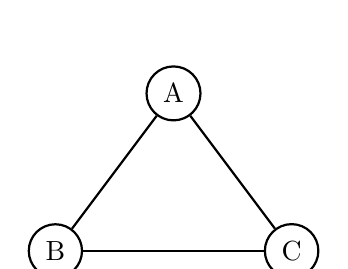
\begin{tikzpicture}
  \node (B) [circle, draw=black, thick, minimum width = 6mm] at (0,0) {B};
  \node (C) [circle, draw=black, thick, minimum width = 6mm] at (3,0) {C};
  \node (A) [circle, draw=black, thick, minimum width = 6mm] at (1.5,2) {A};
  
  \path [-] [thick]
  (A) edge node {} (B)
  (B) edge node {} (C)
  (C) edge node {} (A);
  \end{tikzpicture}
  \caption{A graph G.}
\end{subfigure}
\begin{subfigure}[t]{0.3\textwidth}
\centering
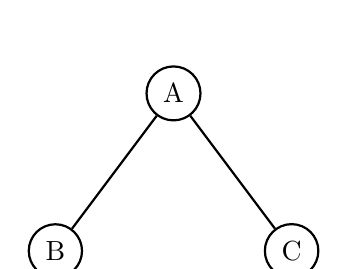
\begin{tikzpicture}
  \node (B) [circle, draw=black, thick, minimum width = 6mm] at (0,0) {B};
  \node (C) [circle, draw=black, thick, minimum width = 6mm] at (3,0) {C};
  \node (A) [circle, draw=black, thick, minimum width = 6mm] at (1.5,2) {A};
  
  \path [-] [thick]
  (A) edge node {} (B)
  (C) edge node {} (A);
\end{tikzpicture}
\caption{The tree given by BFS.}
\end{subfigure}
\begin{subfigure}[t]{0.3\textwidth}
\centering
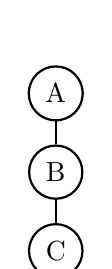
\begin{tikzpicture}
  \node (B) [circle, draw=black, thick, minimum width = 6mm] at (0,1) {B};
  \node (C) [circle, draw=black, thick, minimum width = 6mm] at (0,0) {C};
  \node (A) [circle, draw=black, thick, minimum width = 6mm] at (0,2) {A};
  
  \path [-] [thick]
  (A) edge node {} (B)
  (B) edge node {} (C);
\end{tikzpicture}
\caption{The tree given by DFS.}
\end{subfigure}

\caption{Example of the trees resulting from BFS and DFS. Notice that for a cyclic graph, the tree are different.}
\end{figure*}

\begin{figure*}[!htpb]
\centering
\begin{subfigure}[t]{0.3\textwidth}
\centering
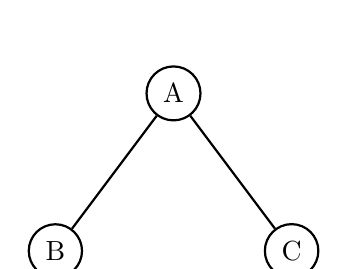
\begin{tikzpicture}
  \node (B) [circle, draw=black, thick, minimum width = 6mm] at (0,0) {B};
  \node (C) [circle, draw=black, thick, minimum width = 6mm] at (3,0) {C};
  \node (A) [circle, draw=black, thick, minimum width = 6mm] at (1.5,2) {A};
  
  \path [-] [thick]
  (A) edge node {} (B)
  (C) edge node {} (A);
  \end{tikzpicture}
  \caption{A graph G.}
\end{subfigure}
\begin{subfigure}[t]{0.3\textwidth}
\centering
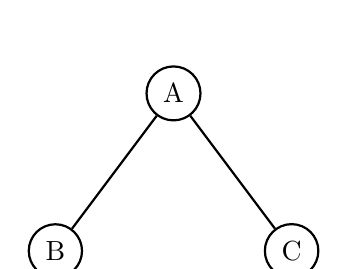
\begin{tikzpicture}
  \node (B) [circle, draw=black, thick, minimum width = 6mm] at (0,0) {B};
  \node (C) [circle, draw=black, thick, minimum width = 6mm] at (3,0) {C};
  \node (A) [circle, draw=black, thick, minimum width = 6mm] at (1.5,2) {A};
  
  \path [-] [thick]
  (A) edge node {} (B)
  (C) edge node {} (A);
\end{tikzpicture}
\caption{The tree given by BFS.}
\end{subfigure}
\begin{subfigure}[t]{0.3\textwidth}
\centering
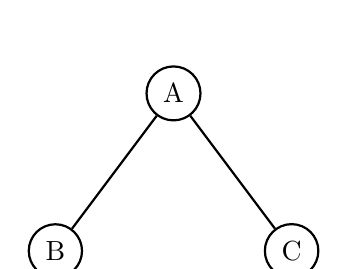
\begin{tikzpicture}
  \node (B) [circle, draw=black, thick, minimum width = 6mm] at (0,0) {B};
  \node (C) [circle, draw=black, thick, minimum width = 6mm] at (3,0) {C};
  \node (A) [circle, draw=black, thick, minimum width = 6mm] at (1.5,2) {A};
  
  \path [-] [thick]
  (A) edge node {} (B)
  (C) edge node {} (A);
\end{tikzpicture}
\caption{The tree given by DFS.}
\end{subfigure}

\caption{Example of the trees resulting from BFS and DFS. Notice that for an acyclic graph, the tree are identical. This example holds for more complex graphs - the only difference is the order in which the tree is produced. In any case, the resulting tree T is the same and is equivalent to G.}
\end{figure*}

\clearpage

\question{Q2}{}
\part{a}
This question is an example of a case where we want to identify max bipartite matching. We set up the graph in the manner shown in Figure 3.

\begin{figure}[!htbp]
\centering
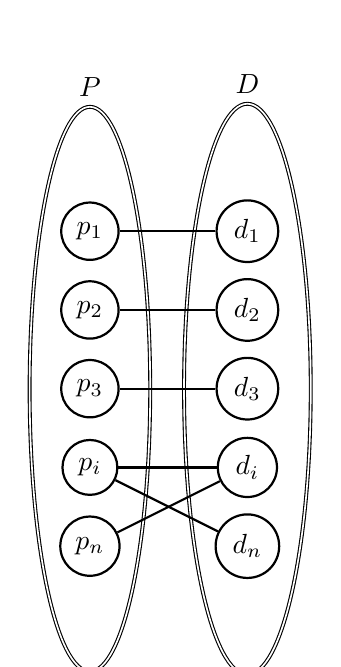
\begin{tikzpicture}
  \node (p1) [circle, draw=black, thick, minimum width = 6mm] at (2,4) {$p_1$};
  \node (p2) [circle, draw=black, thick, minimum width = 6mm] at (2,3) {$p_2$};
  \node (p3) [circle, draw=black, thick, minimum width = 6mm] at (2,2) {$p_3$};
  \node (pi) [circle, draw=black, thick, minimum width = 6mm] at (2,1) {$p_i$};
  \node (pn) [circle, draw=black, thick, minimum width = 6mm] at (2,0) {$p_n$};
  
  \node (d1) [circle, draw=black, thick, minimum width = 6mm] at (4,4) {$d_1$};
  \node (d2) [circle, draw=black, thick, minimum width = 6mm] at (4,3) {$d_2$};
  \node (d3) [circle, draw=black, thick, minimum width = 6mm] at (4,2) {$d_3$};
  \node (di) [circle, draw=black, thick, minimum width = 6mm] at (4,1) {$d_i$};
  \node (dn) [circle, draw=black, thick, minimum width = 6mm] at (4,0) {$d_n$};  
  
  \node[draw=black,double,fit=(p1) (pn) ,inner sep=1ex,ellipse,label=above:$P$] {};
  \node[draw=black,double,fit=(d1) (dn) ,inner sep=1ex,ellipse,label=above:$D$] {};
  
  \path [-] [thick]
  (p1) edge node {} (d1)
  (p2) edge node {} (d2)
  (p3) edge node {} (d3)
  (pi) edge node {} (di)
  (pi) edge node {} (dn)
  (pn) edge node {} (di);
\end{tikzpicture}
\caption{An example of a bipartite graph for this problem.}
\end{figure}

Now, we can solve this as a maximum flow problem using the Ford-Fulkerson method. See Figure 4.

\begin{figure}[!htbp]
\centering
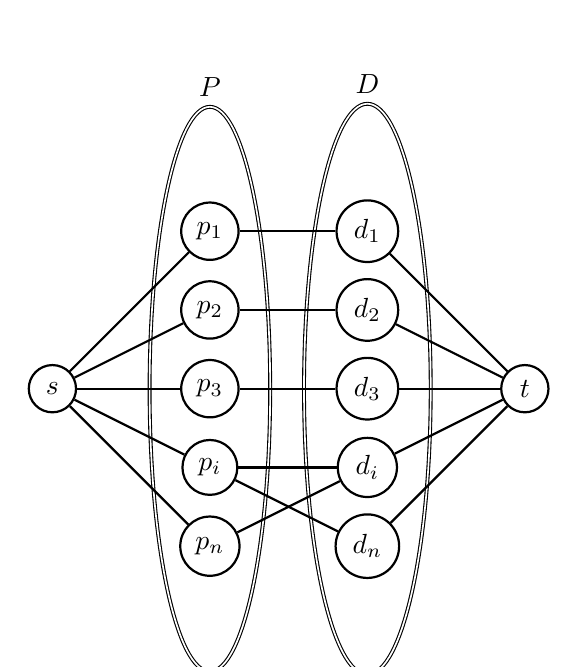
\begin{tikzpicture}
  \node (p1) [circle, draw=black, thick, minimum width = 6mm] at (2,4) {$p_1$};
  \node (p2) [circle, draw=black, thick, minimum width = 6mm] at (2,3) {$p_2$};
  \node (p3) [circle, draw=black, thick, minimum width = 6mm] at (2,2) {$p_3$};
  \node (pi) [circle, draw=black, thick, minimum width = 6mm] at (2,1) {$p_i$};
  \node (pn) [circle, draw=black, thick, minimum width = 6mm] at (2,0) {$p_n$};
  
  \node (d1) [circle, draw=black, thick, minimum width = 6mm] at (4,4) {$d_1$};
  \node (d2) [circle, draw=black, thick, minimum width = 6mm] at (4,3) {$d_2$};
  \node (d3) [circle, draw=black, thick, minimum width = 6mm] at (4,2) {$d_3$};
  \node (di) [circle, draw=black, thick, minimum width = 6mm] at (4,1) {$d_i$};
  \node (dn) [circle, draw=black, thick, minimum width = 6mm] at (4,0) {$d_n$};  
  
  \node (s) [circle, draw=black, thick, minimum width = 6mm] at (0,2) {$s$};
  \node (t) [circle, draw=black, thick, minimum width = 6mm] at (6,2) {$t$};
  
  \node[draw=black,double,fit=(p1) (pn) ,inner sep=1ex,ellipse,label=above:$P$] {};
  \node[draw=black,double,fit=(d1) (dn) ,inner sep=1ex,ellipse,label=above:$D$] {};
  
  \path [-] [thick]
  (p1) edge node {} (s)
  (p2) edge node {} (s)
  (p3) edge node {} (s)
  (pi) edge node {} (s)
  (pn) edge node {} (s)
  (d1) edge node {} (t)
  (d2) edge node {} (t)
  (d3) edge node {} (t)
  (di) edge node {} (t)
  (dn) edge node {} (t)
  (p1) edge node {} (d1)
  (p2) edge node {} (d2)
  (p3) edge node {} (d3)
  (pi) edge node {} (di)
  (pi) edge node {} (dn)
  (pn) edge node {} (di);
\end{tikzpicture}
\caption{The graph G modified to be solved via the Ford-Fulkerson method. Each edge has a capacity of one.}
\end{figure}

If there is a perfect dinner schedule, then there will be perfect and maximum matching. That is, the max flow will be of magnitude $n$. See Figure 5.

\begin{figure}[!htbp]
\centering
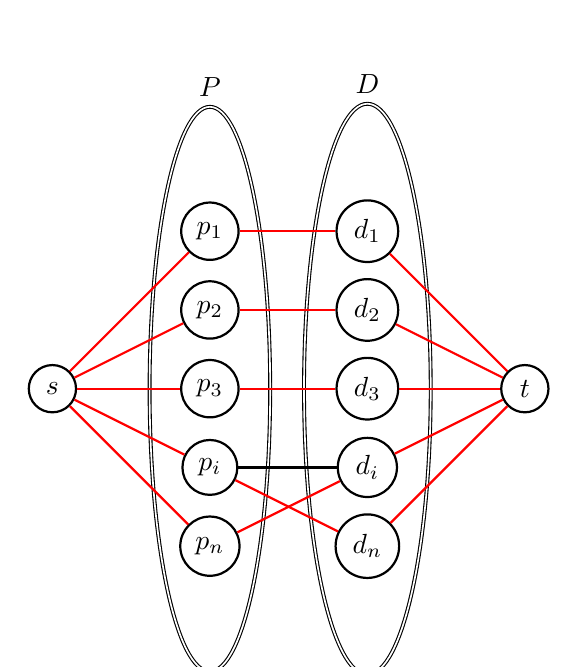
\begin{tikzpicture}
  \node (p1) [circle, draw=black, thick, minimum width = 6mm] at (2,4) {$p_1$};
  \node (p2) [circle, draw=black, thick, minimum width = 6mm] at (2,3) {$p_2$};
  \node (p3) [circle, draw=black, thick, minimum width = 6mm] at (2,2) {$p_3$};
  \node (pi) [circle, draw=black, thick, minimum width = 6mm] at (2,1) {$p_i$};
  \node (pn) [circle, draw=black, thick, minimum width = 6mm] at (2,0) {$p_n$};
  
  \node (d1) [circle, draw=black, thick, minimum width = 6mm] at (4,4) {$d_1$};
  \node (d2) [circle, draw=black, thick, minimum width = 6mm] at (4,3) {$d_2$};
  \node (d3) [circle, draw=black, thick, minimum width = 6mm] at (4,2) {$d_3$};
  \node (di) [circle, draw=black, thick, minimum width = 6mm] at (4,1) {$d_i$};
  \node (dn) [circle, draw=black, thick, minimum width = 6mm] at (4,0) {$d_n$};  
  
  \node (s) [circle, draw=black, thick, minimum width = 6mm] at (0,2) {$s$};
  \node (t) [circle, draw=black, thick, minimum width = 6mm] at (6,2) {$t$};
  
  \node[draw=black,double,fit=(p1) (pn) ,inner sep=1ex,ellipse,label=above:$P$] {};
  \node[draw=black,double,fit=(d1) (dn) ,inner sep=1ex,ellipse,label=above:$D$] {};
  
  \path [-] [thick]
  (p1) edge[red] node {} (s)
  (p2) edge[red] node {} (s)
  (p3) edge[red] node {} (s)
  (pi) edge[red] node {} (s)
  (pn) edge[red] node {} (s)
  (d1) edge[red] node {} (t)
  (d2) edge[red] node {} (t)
  (d3) edge[red] node {} (t)
  (di) edge[red] node {} (t)
  (dn) edge[red] node {} (t)
  (p1) edge[red] node {} (d1)
  (p2) edge[red] node {} (d2)
  (p3) edge[red] node {} (d3)
  (pi) edge node {} (di)
  (pi) edge[red] node {} (dn)
  (pn) edge[red] node {} (di);
\end{tikzpicture}
\caption{Perfect matching of the bipartite graph, and a perfect dinner schedule!}
\end{figure}

\part{b}
We want to see if a perfect matching is possible. With Alanis's schedule, if a perfect matching is possible, then at least one of the edges $(p_i,d_k)$ and $(p_j,d_k)$ that are being used are not needed. Thus, we can do the following. We can evaluate two cases - one with $(p_i,d_k)$ removed and one with $(p_j,d_k)$ removed - and see if an augmenting path can be found in either case. If an augmenting path can be found from either case, then a perfect matching is possible and is produced in $O(n^2)$ time. The complexity is $O(n^2)$ because the number of people and days are equal, and there can be at most $n$ edges for each of $n$ people, resulting in $n^2$ possible edges to evaluate. See Figure 6 for an example of this.

\begin{figure*}[!htpb]
\centering
\begin{subfigure}[t]{0.5\textwidth}
\centering
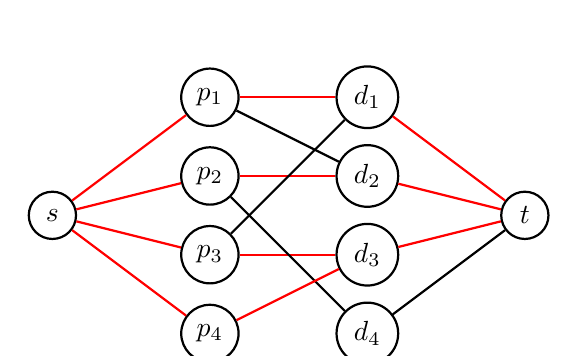
\begin{tikzpicture}
  \node (p1) [circle, draw=black, thick, minimum width = 6mm] at (2,3) {$p_1$};
  \node (p2) [circle, draw=black, thick, minimum width = 6mm] at (2,2) {$p_2$};
  \node (p3) [circle, draw=black, thick, minimum width = 6mm] at (2,1) {$p_3$};
  \node (p4) [circle, draw=black, thick, minimum width = 6mm] at (2,0) {$p_4$};
  
  \node (d1) [circle, draw=black, thick, minimum width = 6mm] at (4,3) {$d_1$};
  \node (d2) [circle, draw=black, thick, minimum width = 6mm] at (4,2) {$d_2$};
  \node (d3) [circle, draw=black, thick, minimum width = 6mm] at (4,1) {$d_3$};
  \node (d4) [circle, draw=black, thick, minimum width = 6mm] at (4,0) {$d_4$};
  
  \node (s) [circle, draw=black, thick, minimum width = 6mm] at (0,1.5) {$s$};
  \node (t) [circle, draw=black, thick, minimum width = 6mm] at (6,1.5) {$t$};
  
  \path [-] [thick]
  (p1) edge[red] node {} (s)
  (p2) edge[red] node {} (s)
  (p3) edge[red] node {} (s)
  (p4) edge[red] node {} (s)
  (d1) edge[red] node {} (t)
  (d2) edge[red] node {} (t)
  (d3) edge[red] node {} (t)
  (d4) edge node {} (t)
  (p1) edge[red] node {} (d1)
  (p2) edge[red] node {} (d2)
  (p3) edge[red] node {} (d3)
  (p1) edge node {} (d2)
  (p2) edge node {} (d4)
  (p3) edge node {} (d1)
  (p4) edge[red] node {} (d3);
\end{tikzpicture}
\caption{The schedule proposed by Alanis.}
\end{subfigure}%
\begin{subfigure}[t]{0.5\textwidth}
\centering
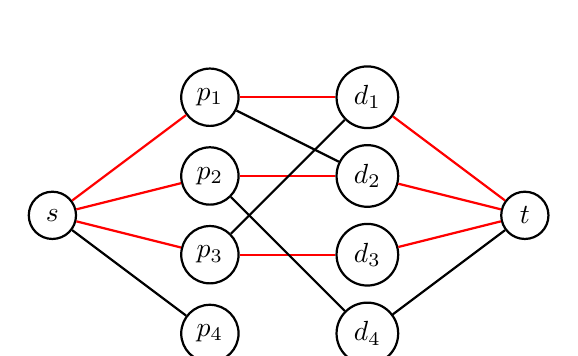
\begin{tikzpicture}
  \node (p1) [circle, draw=black, thick, minimum width = 6mm] at (2,3) {$p_1$};
  \node (p2) [circle, draw=black, thick, minimum width = 6mm] at (2,2) {$p_2$};
  \node (p3) [circle, draw=black, thick, minimum width = 6mm] at (2,1) {$p_3$};
  \node (p4) [circle, draw=black, thick, minimum width = 6mm] at (2,0) {$p_4$};
  
  \node (d1) [circle, draw=black, thick, minimum width = 6mm] at (4,3) {$d_1$};
  \node (d2) [circle, draw=black, thick, minimum width = 6mm] at (4,2) {$d_2$};
  \node (d3) [circle, draw=black, thick, minimum width = 6mm] at (4,1) {$d_3$};
  \node (d4) [circle, draw=black, thick, minimum width = 6mm] at (4,0) {$d_4$};
  
  \node (s) [circle, draw=black, thick, minimum width = 6mm] at (0,1.5) {$s$};
  \node (t) [circle, draw=black, thick, minimum width = 6mm] at (6,1.5) {$t$};
  
  \path [-] [thick]
  (p1) edge[red] node {} (s)
  (p2) edge[red] node {} (s)
  (p3) edge[red] node {} (s)
  (p4) edge node {} (s)
  (d1) edge[red] node {} (t)
  (d2) edge[red] node {} (t)
  (d3) edge[red] node {} (t)
  (d4) edge node {} (t)
  (p1) edge[red] node {} (d1)
  (p2) edge[red] node {} (d2)
  (p3) edge[red] node {} (d3)
  (p1) edge node {} (d2)
  (p2) edge node {} (d4)
  (p3) edge node {} (d1);
\end{tikzpicture}
\caption{Case 1 - Remove edge $(p_4,d_3)$. No augmenting path exists.}
\end{subfigure}

\begin{subfigure}[t]{0.5\textwidth}
\centering
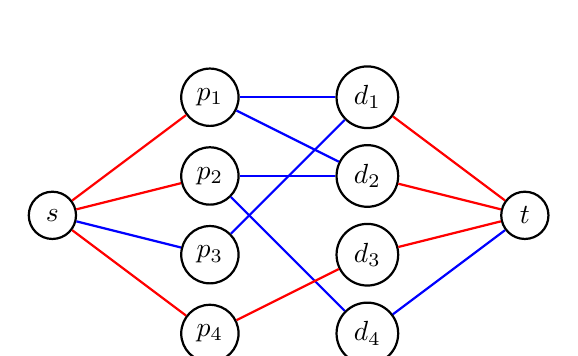
\begin{tikzpicture}
  \node (p1) [circle, draw=black, thick, minimum width = 6mm] at (2,3) {$p_1$};
  \node (p2) [circle, draw=black, thick, minimum width = 6mm] at (2,2) {$p_2$};
  \node (p3) [circle, draw=black, thick, minimum width = 6mm] at (2,1) {$p_3$};
  \node (p4) [circle, draw=black, thick, minimum width = 6mm] at (2,0) {$p_4$};
  
  \node (d1) [circle, draw=black, thick, minimum width = 6mm] at (4,3) {$d_1$};
  \node (d2) [circle, draw=black, thick, minimum width = 6mm] at (4,2) {$d_2$};
  \node (d3) [circle, draw=black, thick, minimum width = 6mm] at (4,1) {$d_3$};
  \node (d4) [circle, draw=black, thick, minimum width = 6mm] at (4,0) {$d_4$};
  
  \node (s) [circle, draw=black, thick, minimum width = 6mm] at (0,1.5) {$s$};
  \node (t) [circle, draw=black, thick, minimum width = 6mm] at (6,1.5) {$t$};
  
  \path [-] [thick]
  (p1) edge[red] node {} (s)
  (p2) edge[red] node {} (s)
  (p3) edge[blue] node {} (s)
  (p4) edge[red] node {} (s)
  (d1) edge[red] node {} (t)
  (d2) edge[red] node {} (t)
  (d3) edge[red] node {} (t)
  (d4) edge[blue] node {} (t)
  (p1) edge[blue] node {} (d1)
  (p2) edge[blue] node {} (d2)
  (p1) edge[blue] node {} (d2)
  (p2) edge[blue] node {} (d4)
  (p3) edge[blue] node {} (d1)
  (p4) edge[red] node {} (d3);
\end{tikzpicture}
\caption{Case 2 - Remove edge $(p_3,d_3)$. An augmenting path does exist (shown in blue).}
\end{subfigure}%
\begin{subfigure}[t]{0.5\textwidth}
\centering
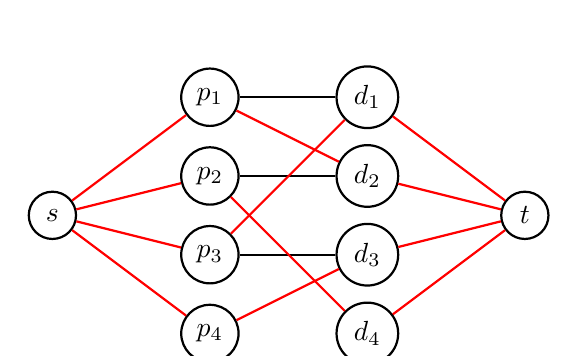
\begin{tikzpicture}
  \node (p1) [circle, draw=black, thick, minimum width = 6mm] at (2,3) {$p_1$};
  \node (p2) [circle, draw=black, thick, minimum width = 6mm] at (2,2) {$p_2$};
  \node (p3) [circle, draw=black, thick, minimum width = 6mm] at (2,1) {$p_3$};
  \node (p4) [circle, draw=black, thick, minimum width = 6mm] at (2,0) {$p_4$};
  
  \node (d1) [circle, draw=black, thick, minimum width = 6mm] at (4,3) {$d_1$};
  \node (d2) [circle, draw=black, thick, minimum width = 6mm] at (4,2) {$d_2$};
  \node (d3) [circle, draw=black, thick, minimum width = 6mm] at (4,1) {$d_3$};
  \node (d4) [circle, draw=black, thick, minimum width = 6mm] at (4,0) {$d_4$};
  
  \node (s) [circle, draw=black, thick, minimum width = 6mm] at (0,1.5) {$s$};
  \node (t) [circle, draw=black, thick, minimum width = 6mm] at (6,1.5) {$t$};
  
  \path [-] [thick]
  (p1) edge[red] node {} (s)
  (p2) edge[red] node {} (s)
  (p3) edge[red] node {} (s)
  (p4) edge[red] node {} (s)
  (d1) edge[red] node {} (t)
  (d2) edge[red] node {} (t)
  (d3) edge[red] node {} (t)
  (d4) edge[red] node {} (t)
  (p1) edge node {} (d1)
  (p2) edge node {} (d2)
  (p3) edge node {} (d3)
  (p1) edge[red] node {} (d2)
  (p2) edge[red] node {} (d4)
  (p3) edge[red] node {} (d1)
  (p4) edge[red] node {} (d3);
\end{tikzpicture}
\caption{The resulting perfect schedule!}
\end{subfigure}
\caption{Example of correcting an ``almost perfect'' schedule.}
\end{figure*}

\clearpage

\question{Q3}{}
Here I present a modified BFS algorithm to determine whether or not a virus introduced to computer $C_a$ at time $x$ could have infected computer $C_b$ by time $y$.
\begin{lstlisting}
ModifiedBFS(G, Ca, x, Cb, y){
	// Set all nodes beside root to default settings
	for (u in G.V - {s}){
		u.color = white;
		u.parent = null;
		u.time = null;
	}
	
	// Set root node settings
	Ca.color = red;
	Ca.parent = new ArrayList();
	Ca.time = x;
	
	// Create queue and add Ca
	Q = 0;
	Enqueue(Q,Ca);
	
	// Primary loop
	while (Q != 0){
		u = Dequeue(Q);
		for (v in G.Adj[u] - {u.parent}){
			if (v.color == white){
				if (w(u,v) >= u.time){
					v.color = red;
					v.parent = append(u);
					v.time = w(u,v);
					Enqueue(Q,v);
				}
			}
			if (v.color == red){
				if (w(u,v) >= u.time && w(u,v) < v.time){
					v.parent = append(u);
					v.time = w(u,v);
					Enqueue(Q,v);
				}
			}
	
	// Check if $C_b$ is infected at time $y$
	if (Cb.color == red && Cb.time <= y){
		return true;
	}
	else{
		return false;
	}
}		
\end{lstlisting}

This is a modified BFS algorithm, in which infected nodes are set to color=red and noninfected nodes are color=white. Each node has an associated time of infection and an ArrayList of "parents", which keeps track of nodes which it could have been infected from.

If a node is white, and if the edge weight is $\geq$ the infection time of the parent, then it will be set as follows: color=red, parent=append(u), time=w(u,v). Then it will be added to the queue. Only infected nodes are added to the queue.

If a node is red, and if the edge weight is $\geq$ the infection time of the parent \textit{and} the edge weight is $<$ its current infection time, then it will be updated as follows: parent=append(u), time=w(u,v). Then it will be added to the queue. See Figure 7 for an example.

\begin{figure*}[!htpb]
\centering
\begin{subfigure}[t]{0.3\textwidth}
\centering
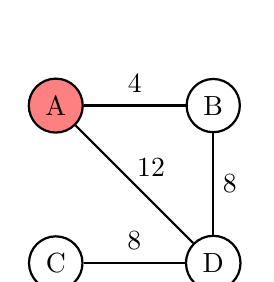
\begin{tikzpicture}
  \node (A) [fill=red!50, circle, draw=black, thick, minimum width = 6mm] at (0,2) {A};
  \node (B) [circle, draw=black, thick, minimum width = 6mm] at (2,2) {B};
  \node (C) [circle, draw=black, thick, minimum width = 6mm] at (0,0) {C};
  \node (D) [circle, draw=black, thick, minimum width = 6mm] at (2,0) {D};
  
  \path [-] [thick]
  (A) edge node [yshift=8pt]{4} (B)
  (B) edge node [xshift=6pt]{8} (D)
  (C) edge node [yshift=8pt]{8} (D)
  (A) edge node [xshift=6pt,yshift=6pt]{12} (D);
  \end{tikzpicture}
  \caption{}
\end{subfigure}
\begin{subfigure}[t]{0.3\textwidth}
\centering
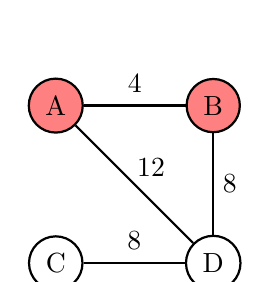
\begin{tikzpicture}
  \node (A) [fill=red!50, circle, draw=black, thick, minimum width = 6mm] at (0,2) {A};
  \node (B) [fill=red!50, circle, draw=black, thick, minimum width = 6mm] at (2,2) {B};
  \node (C) [circle, draw=black, thick, minimum width = 6mm] at (0,0) {C};
  \node (D) [circle, draw=black, thick, minimum width = 6mm] at (2,0) {D};
  
  \path [-] [thick]
  (A) edge node [yshift=8pt]{4} (B)
  (B) edge node [xshift=6pt]{8} (D)
  (C) edge node [yshift=8pt]{8} (D)
  (A) edge node [xshift=6pt,yshift=6pt]{12} (D);
  \end{tikzpicture}
\caption{}
\end{subfigure}
\begin{subfigure}[t]{0.3\textwidth}
\centering
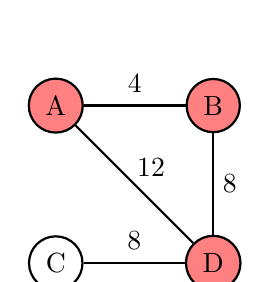
\begin{tikzpicture}
  \node (A) [fill=red!50, circle, draw=black, thick, minimum width = 6mm] at (0,2) {A};
  \node (B) [fill=red!50, circle, draw=black, thick, minimum width = 6mm] at (2,2) {B};
  \node (C) [circle, draw=black, thick, minimum width = 6mm] at (0,0) {C};
  \node (D) [fill=red!50, circle, draw=black, thick, minimum width = 6mm] at (2,0) {D};
  
  \path [-] [thick]
  (A) edge node [yshift=8pt]{4} (B)
  (B) edge node [xshift=6pt]{8} (D)
  (C) edge node [yshift=8pt]{8} (D)
  (A) edge node [xshift=6pt,yshift=6pt]{12} (D);
  \end{tikzpicture}
\caption{}
\end{subfigure}

\begin{subfigure}[t]{0.3\textwidth}
\centering
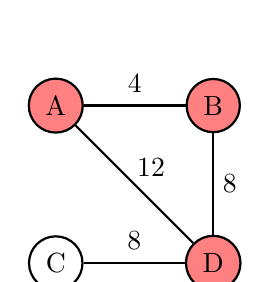
\begin{tikzpicture}
  \node (A) [fill=red!50, circle, draw=black, thick, minimum width = 6mm] at (0,2) {A};
  \node (B) [fill=red!50, circle, draw=black, thick, minimum width = 6mm] at (2,2) {B};
  \node (C) [circle, draw=black, thick, minimum width = 6mm] at (0,0) {C};
  \node (D) [fill=red!50, circle, draw=black, thick, minimum width = 6mm] at (2,0) {D};
  
  \path [-] [thick]
  (A) edge node [yshift=8pt]{4} (B)
  (B) edge node [xshift=6pt]{8} (D)
  (C) edge node [yshift=8pt]{8} (D)
  (A) edge node [xshift=6pt,yshift=6pt]{12} (D);
  \end{tikzpicture}
\caption{}
\end{subfigure}
\begin{subfigure}[t]{0.3\textwidth}
\centering
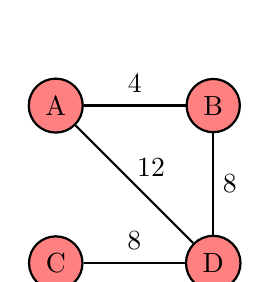
\begin{tikzpicture}
  \node (A) [fill=red!50, circle, draw=black, thick, minimum width = 6mm] at (0,2) {A};
  \node (B) [fill=red!50, circle, draw=black, thick, minimum width = 6mm] at (2,2) {B};
  \node (C) [fill=red!50, circle, draw=black, thick, minimum width = 6mm] at (0,0) {C};
  \node (D) [fill=red!50, circle, draw=black, thick, minimum width = 6mm] at (2,0) {D};
  
  \path [-] [thick]
  (A) edge node [yshift=8pt]{4} (B)
  (B) edge node [xshift=6pt]{8} (D)
  (C) edge node [yshift=8pt]{8} (D)
  (A) edge node [xshift=6pt,yshift=6pt]{12} (D);
  \end{tikzpicture}
\caption{}
\end{subfigure}

\caption{An example of the Modified BFS algorithm. In (a), the initial conditions are presented. Time of infection of Node A is 2. In (b), Node B is examined. Because the edge weight is greater than 2, Node B is infected at time 4. In (c), Node D is examined. Because the edge weight is greater than 2, Node D is infected at time 12. In (d), we move on to Node B as the ``root'' node. Because Node A is a parent of Node B, it is not examined, and only Node D is examined. Because the weight of the edge is greater than 4, but less than 12, the time of infection for Node D is updated to the weight of the edge BD, or 8. In (e), we move on to Node D as the ``root'' node. Because both Node A and Node B are retained as parents, neither is examined. Only Node C is examined. Because the edge weight is greater or equal to 8, Node C is infected at time 8. At this point, all edges have been examined once ($m$ times), and the function returns true or false based on input.}
\end{figure*}

We can show that this algorithm runs in $O(m)$ time because each triple represents an edge, and there are $m$ triples. We are examining only edges that have not been examined before, so at most $m$ edges. Figure 7d highlights this point. The cost of the queue operations and the setting of initial conditions operates only on the nodes, and there will be at most $\lvert E \rvert+1$ nodes.

\clearpage

\question{Q4}{}
\part{a}
This is similar to Problem 2 of this assignment. The best approach here is two set up two disjoint sets $X$ and $S$, a source node $s$ and a sink node $t$. There can be other nodes outside of these presented, but there can only be one output edge from each node in $X$. All edges except those from nodes in $S$ to $t$ must have a capacity of one. Edges from nodes in $S$ to $t$ have a capacity of $\lvert X \rvert$. Construct a graph $G$ as shown in Figure 8.

\begin{figure}[!htbp]
\centering
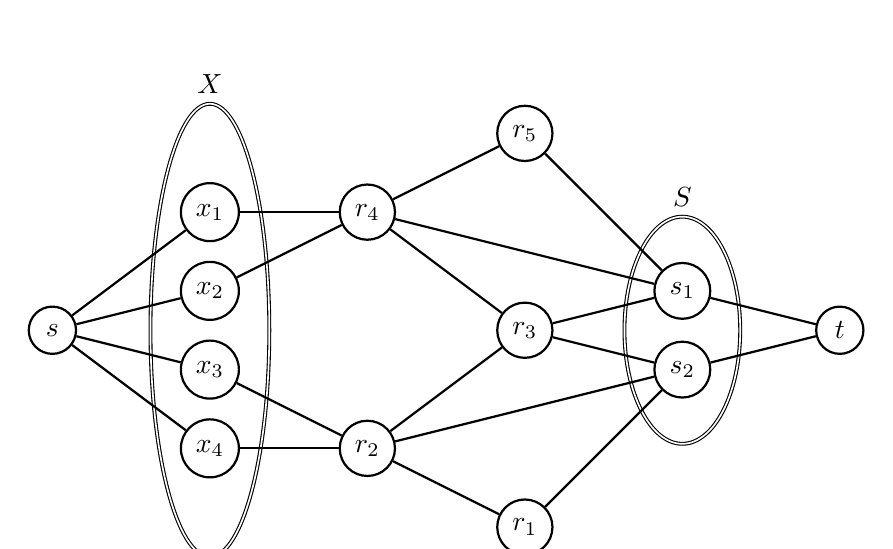
\begin{tikzpicture}
  \node (x1) [circle, draw=black, thick, minimum width = 6mm] at (2,3) {$x_1$};
  \node (x2) [circle, draw=black, thick, minimum width = 6mm] at (2,2) {$x_2$};
  \node (x3) [circle, draw=black, thick, minimum width = 6mm] at (2,1) {$x_3$};
  \node (x4) [circle, draw=black, thick, minimum width = 6mm] at (2,0) {$x_4$};
  
  \node (s1) [circle, draw=black, thick, minimum width = 6mm] at (8,2) {$s_1$};
  \node (s2) [circle, draw=black, thick, minimum width = 6mm] at (8,1) {$s_2$}; 
  
  \node (r1) [circle, draw=black, thick, minimum width = 6mm] at (6,-1) {$r_1$}; 
  \node (r2) [circle, draw=black, thick, minimum width = 6mm] at (4,0) {$r_2$}; 
  \node (r3) [circle, draw=black, thick, minimum width = 6mm] at (6,1.5) {$r_3$}; 
  \node (r4) [circle, draw=black, thick, minimum width = 6mm] at (4,3) {$r_4$}; 
  \node (r5) [circle, draw=black, thick, minimum width = 6mm] at (6,4) {$r_5$};
  
  \node (s) [circle, draw=black, thick, minimum width = 6mm] at (0,1.5) {$s$};
  \node (t) [circle, draw=black, thick, minimum width = 6mm] at (10,1.5) {$t$};
     
  
  \node[draw=black,double,fit=(x1) (x4) ,inner sep=1ex,ellipse,label=above:$X$] {};
  \node[draw=black,double,fit=(s1) (s2) ,inner sep=1ex,ellipse,label=above:$S$] {};
  
  \path [-] [thick]
  (s) edge node {} (x1)
  (s) edge node {} (x2)
  (s) edge node {} (x3)
  (s) edge node {} (x4)
  (x1) edge node {} (r4)
  (x2) edge node {} (r4)
  (x3) edge node {} (r2)
  (x4) edge node {} (r2)
  (r2) edge node {} (r1)
  (r2) edge node {} (r3)
  (r2) edge node {} (s2)
  (r4) edge node {} (r3)
  (r4) edge node {} (r5)
  (r4) edge node {} (s1)
  (r1) edge node {} (s2)
  (r3) edge node {} (s2)
  (r3) edge node {} (s1)
  (r5) edge node {} (s1)
  (s1) edge node {} (t)
  (s2) edge node {} (t);
\end{tikzpicture}
\caption{An example of a graph for this problem.}
\end{figure}

With the graph constructed, solve the Max Flow problem using the Ford-Fulkerson method. If the maximum flow is equal to $\lvert X \rvert$, then a set of routes exists.

\part{b}
While Part A required enforcement of ``edge-disjoint'' rules, this part requires enforcement of ``node-disjoint'' rules. In Figure 8, a set of routes exists when following edge-disjoint rules, but not when following node-disjoint rules. This is because the four nodes of $X$ converge two only two nodes $r_2$ and $r_4$. Thus only two cities would be able to escape if using node-disjoint rules.

To enforce this rule, we must modify our graph $G$. We could create a graph $G'$ in which each of the ``in-between'' nodes $r_i$ are duplicated. One of these duplicate nodes serves as an input, one serves as an output, and an edge of capacity one connects them. It is important that the connecting edge be of capacity one, as this enforces the node-disjoint rule by prohibiting flow from more than one source through the node. This modified graph $G'$ can be solved via the same Ford-Fulkerson method. If the max flow is equal to $\lvert X \rvert$, then a set of routes exists.

\end{document}









